% Unofficial University of Cambridge Poster Template
% https://github.com/andiac/gemini-cam
% a fork of https://github.com/anishathalye/gemini
% also refer to https://github.com/k4rtik/uchicago-poster

\documentclass[final,20pt]{beamer}

% ====================
% Packages
% ====================

\usepackage[T1]{fontenc}
\usepackage{lmodern}
\usepackage[orientation=portrait,size=a0,scale=1.194]{beamerposter}
\usetheme{gemini}
% \usecolortheme{nott}
\usepackage{graphicx}
\usepackage{booktabs}
\usepackage{tikz}
\usepackage{pgfplots}
\pgfplotsset{compat=1.14}
\usepackage{anyfontsize}
\usepackage{svg}
\usepackage[portuguese]{babel}
\usepackage{hyphenat}
\usepackage{tikz} % for overlaying image
\hyphenation{pro-ce-ssa-men-to}

\newcommand{\RA}[1]{{\color{blue} #1}}
% If you have N columns, choose \sepwidth and \colwidth such that
% (N+1)*\sepwidth + N*\colwidth = \paperwidth
\newlength{\sepwidth}
\newlength{\colwidth}
\setlength{\sepwidth}{0.025\paperwidth}
\setlength{\colwidth}{0.45\paperwidth}

\newcommand{\separatorcolumn}{\begin{column}{\sepwidth}\end{column}}

% ====================
% Title
% ====================

\title{ProVant-Emergentia: Projeto de um Sistema Embarcado para VANTs}

\author{Alunos: Luis Gonzalez, Lucas Silveira, Enzo Bahia}

\institute[shortinst]{Orientador: Guilherme V. Raffo, Co-Orientador: Richard Andrade}

% ====================
% Footer (optional)
% ====================

\footercontent{
  \href{https://utfpr.edu.br/ct/ppgca}{utfpr.edu.br/ct/ppgca} \hfill
  Mostra de Trabalhos do PPGCA --- TechTalks 2024 \hfill
  \href{mailto:ppgca-ct@utfpr.edu.br}{ppgca-ct@utfpr.edu.br}}
% (can be left out to remove footer)


% ====================
% Logo (optional)
% ====================

% use this to include logos on the left and/or right side of the header:
\logoleft{
\includegraphics[scale=0.9]{logos/ufmg_wite.pdf}}
\logoright{
\includegraphics[scale=0.9]{logos/macro_logo_wite.pdf}}

% ====================
% Body
% ====================

\begin{document}

% Refer to https://github.com/k4rtik/uchicago-poster
% logo: https://www.cam.ac.uk/brand-resources/about-the-logo/logo-downloads
% \addtobeamertemplate{headline}{}
% {
%     \begin{tikzpicture}[remember picture,overlay]
%       \node [anchor=north west, inner sep=3cm] at ([xshift=-2.5cm,yshift=1.75cm]current page.north west)
%       {\includegraphics[height=7cm]{logos/unott-logo.eps}}; 
%     \end{tikzpicture}
% }

\begin{frame}[t]
\begin{columns}[t]
\separatorcolumn

\begin{column}{\colwidth}

  \begin{block}{Introdução}

    O ProVANT-\textit{Emergentia} consiste num VANT do tipo \textit{tilt-rotor} onde é possível modificar a angulação dos propulsores, permitindo a alternância de modo de voo entre helicóptero e cruzeiro. O uso da aeronave é  destinado a situações de busca e resgate, prezando-se por capacidade de resposta ágil, pouca necessidade de espaço para decolagem e aterrissagem e fácil transporte por um veículo de apoio. Nesse contexto, o projeto do sistema embarcado compreende desde o design da arquitetura de \textit{hardware} do sistema, até o desenvolvimento de \textit{firmware} e fabricação de circuitos dedicados.

    % Aqui ainda não está cabendo o restante do texto. 

  \end{block}
\vspace{-1em}
  \begin{block}{Objetivos}

    O projeto do sistema embarcado do VANT visa:
   
    %\begin{itemize}
    % Comentários feitos anteriormente 

    % \begin{itemize}
    %   \item Suportar um sistema de controle de voo de alto \textbf{desempenho}, com capacidade de operar dentro de uma janela de amostragem de 12 ms.
    %   \item Estabelecer redes de \textbf{comunicação} interna e externa (com a Estação Base) que cumpram com os requisitos de tempo do sistema de controle de voo. 
    %   \item Desenvolver e implementar arquiteturas de \textit{hardware} e \textit{software} tendo como princípios \textbf{modularidade} e \textbf{especialização}, através da divisão em subsistemas.
    %   \item Mitigar e aplicar estratégias de remediação para cenários de falha através do emprego de \textbf{redundância} de funcionalidades e dispositivos e mudança automática no modo de operação, conforme diferentes cenários de falha.
     
    % \end{itemize}

  \end{block}
\vspace{-2em}
  \begin{block}{Projeto de Hardware}

    Quanto a natureza de sua operação, o VANT pode ser compreendido como um \textit{Safety Critical System}, requerendo cuidados extras em relação à redundância de subsistemas críticos, operação em tempo real e garantia de confiabilidade durante a operação.
    Assim, a eletrônica embarcada foi subdivida conforme é mostrado na Figura 1.
    
    % \begin{itemize}
    %   \item \textbf{Subsistema Jetson: } Possui uma Jetson TX2 com GPU dedicada para execução dos algoritmos de controle de alto custo computacional em termos de paralelismo; GPS e  IMU, de alta precisão.
    %   \item \textbf{Subsistema Nucleo: } Possui uma NUCLEO-F767ZI ligada a dois sistemas de barramento: um para leitura dos sensores e outro para controle dos atuadores. Em caso de falha do Subsistema Jetson, pode substituí-lo com controladores mais simples para que a aeronave consiga retornar ao solo. Conta ainda com uma NUCLEO redundante, em caso de queda da principal.
    %   \item \textbf{Subsistema Raspberry: } Possui uma Raspberry Pi 4 com \textit{shield} Navio2®, para execução de um estimador independente redundante ao estimador presente na Jetson; sensor de pressão; sonar e radio-\textit{receiver}. Também realiza a comunicação com a Estação de Solo. 
    %   \item \textbf{Power Supply \& Solar Subsystems: } Esta composto de baterias, módulos conversores, BMS, células fotovoltaicas e circuito de carregamento dedicado. 
    % \end{itemize}

    \begin{figure}
        \centering
        \includesvg[width = 0.9\linewidth]{Figuras/hardware-structure} 
        \caption{Estrutura de Hardware do ProVANT-\textit{Emergentia}}
        \label{fig:hardware-structure}
    \end{figure}

  \end{block}
  \vspace{-2em}
  \begin{block}{Projeto de Software}
   
    \begin{minipage} {0.65\linewidth}
     
         A estrutura do software desenvolvido dada da seguinte forma:
        \begin{itemize}
             \item \textbf{Device Layer}: \textit{drivers} de cada dispositivo do VANT (e.g. sensores e atuadores).
             \item \textbf{Libraries}: software de uso geral, programas de utilidade e funcionalidades comuns a todos os módulos (e.g. comunicação Ethernet)
             \item \textbf{Application}: programas da aplicação final, threads com distintas funcionalidades de leitura de dados, comunicação, etc.
         \end{itemize}
        Existem duas divisões adicionais: software de baixo nível (\textbf{Low Level}), utilizado nos computadores com funcionalidades de GPIO e escrito em linguagem C, e software de alto nível (\textbf{High Level}), utilizado nos computadores de maior capacidade computacional e escrito em C++. 
        
    \end{minipage}
    %\hspace{0.05\linewidth}
    \begin{minipage} {0.3\linewidth}
    
        \includesvg[width = 1.1\linewidth]{Figuras/Project-Software-Arch}
    \end{minipage}
  \end{block}

\end{column}

\begin{column}{\colwidth}
    \vspace{0.5em}
    \begin{minipage} {\linewidth}
    No que diz respeito à aplicação particular do ProVant-Emergentia, os programas são organizados em \textit{threads} divididas de acordo com a sua funcionalidade: i) \textbf{processamento de dados} de sensores e atuadores; ii) \textbf{comunicação em rede}; iii) \textbf{algoritmos de controle}; e iv) \textbf{telemetria} para a \textit{Groundstation}.
   
    % Para comunicar os distintos computadores de bordo, foi elaborado um protocolo de comunicação próprio com arquitetura \textbf{Token Ring}, de maneira a aproveitar o alto fluxo de dados de conexões Ethernet ao mesmo tempo em que as colisões de pacotes e o não-determinismo temporal gerado pelo mecanismo CSMA-CD é mitigado. Esse mecanismo é mostrado de forma resumida na Figura \ref{fig:hardware-structure}, onde é possível ver o fluxo de comunicação dos computadores de bordo. 
     \end{minipage}
  \begin{block}{Implementação}
    
    % O desenvolvimento do hardware ocorreu inicialmente com a integração de todos os sistemas embarcados, sensores e atuadores do VANT através decircuitos impressos servindo como barramentos. 
    % Quatro circuitos principais foram projetados: i) O circuito \textit{Sensor Bus} que conecta os embarcados aos sensores; ii) o \textit{Actuator Bus} que conecta os embarcados aos atuadores; iii) a \textit{Nucleo Shield} que conecta as placas NUCLEO-F767ZI a outros circuitos; iV) e a \textit{Jetson Shield} que conecta a placa Jetson TX2 à IMU ADIS e o módulo de GPS C099-F9P. 
    % Para a manufatura dos circuitos impressos utilizamos o softtware EAGLE para o projeto e uma máquina CNC para a produção das placas impressas. Os circuitos permitem a alimentação de energia dos componentes eletrônicos e a comunicação entre os computadores embarcados e os sensores e atuadores, enquanto a comunicação entre os embarcados é feita através de estrutura baseada em ETHERNET.
    
        \begin{minipage} {0.5\linewidth}
        \begin{figure}
            \centering
            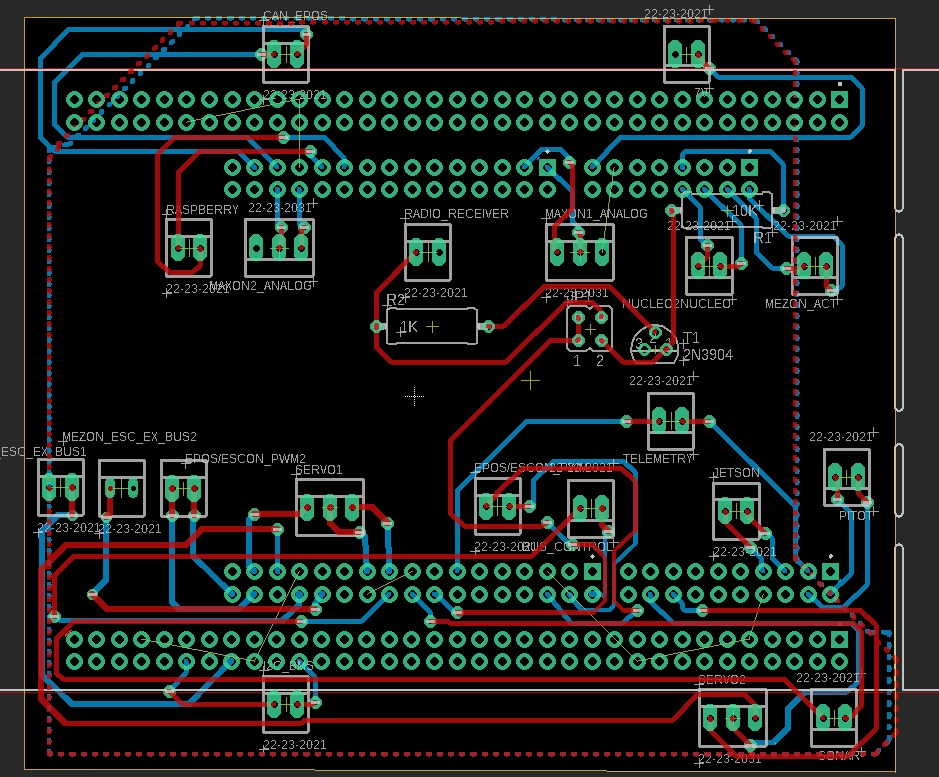
\includegraphics[width=0.75\linewidth]{Figuras/EAGLE.jpeg}
            \caption{Design do circuito impresso no EAGLE}
            \label{fig:enter-label}
        \end{figure}
    \end{minipage}
    \begin{minipage} {0.5\linewidth}
        \begin{figure}
            \centering
            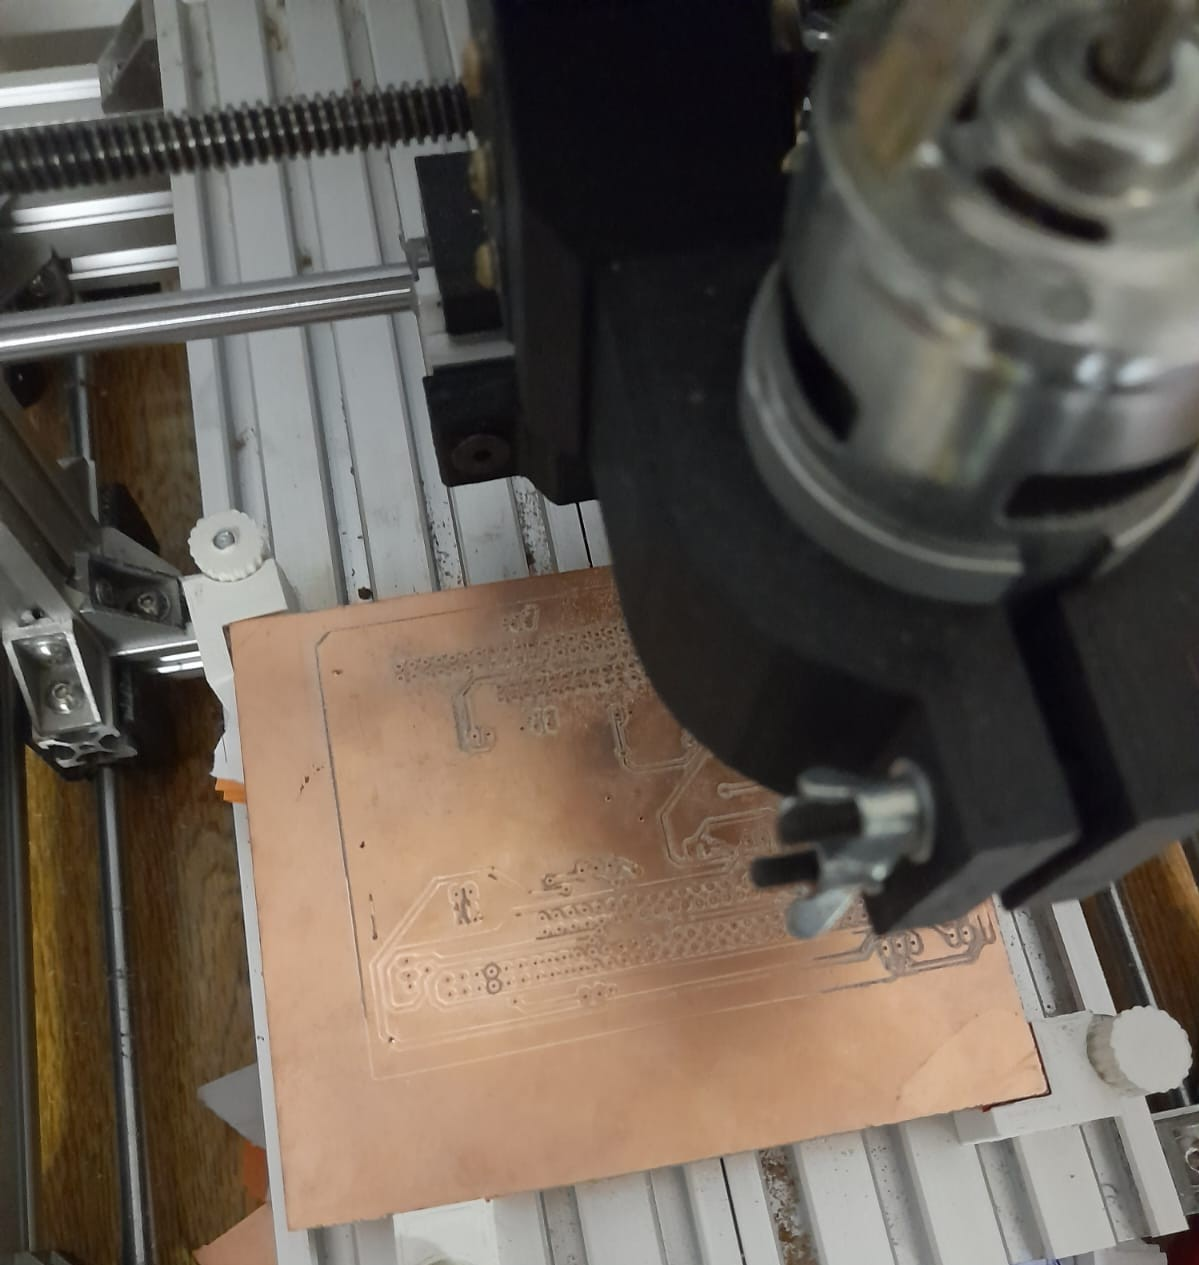
\includegraphics[width=0.58\linewidth]{Figuras/CNC.jpeg}
            \caption{Criação do circuito na máquina CNC}
            \label{fig:enter-label}
        \end{figure}
    \end{minipage}
    \begin{figure}
        \centering
        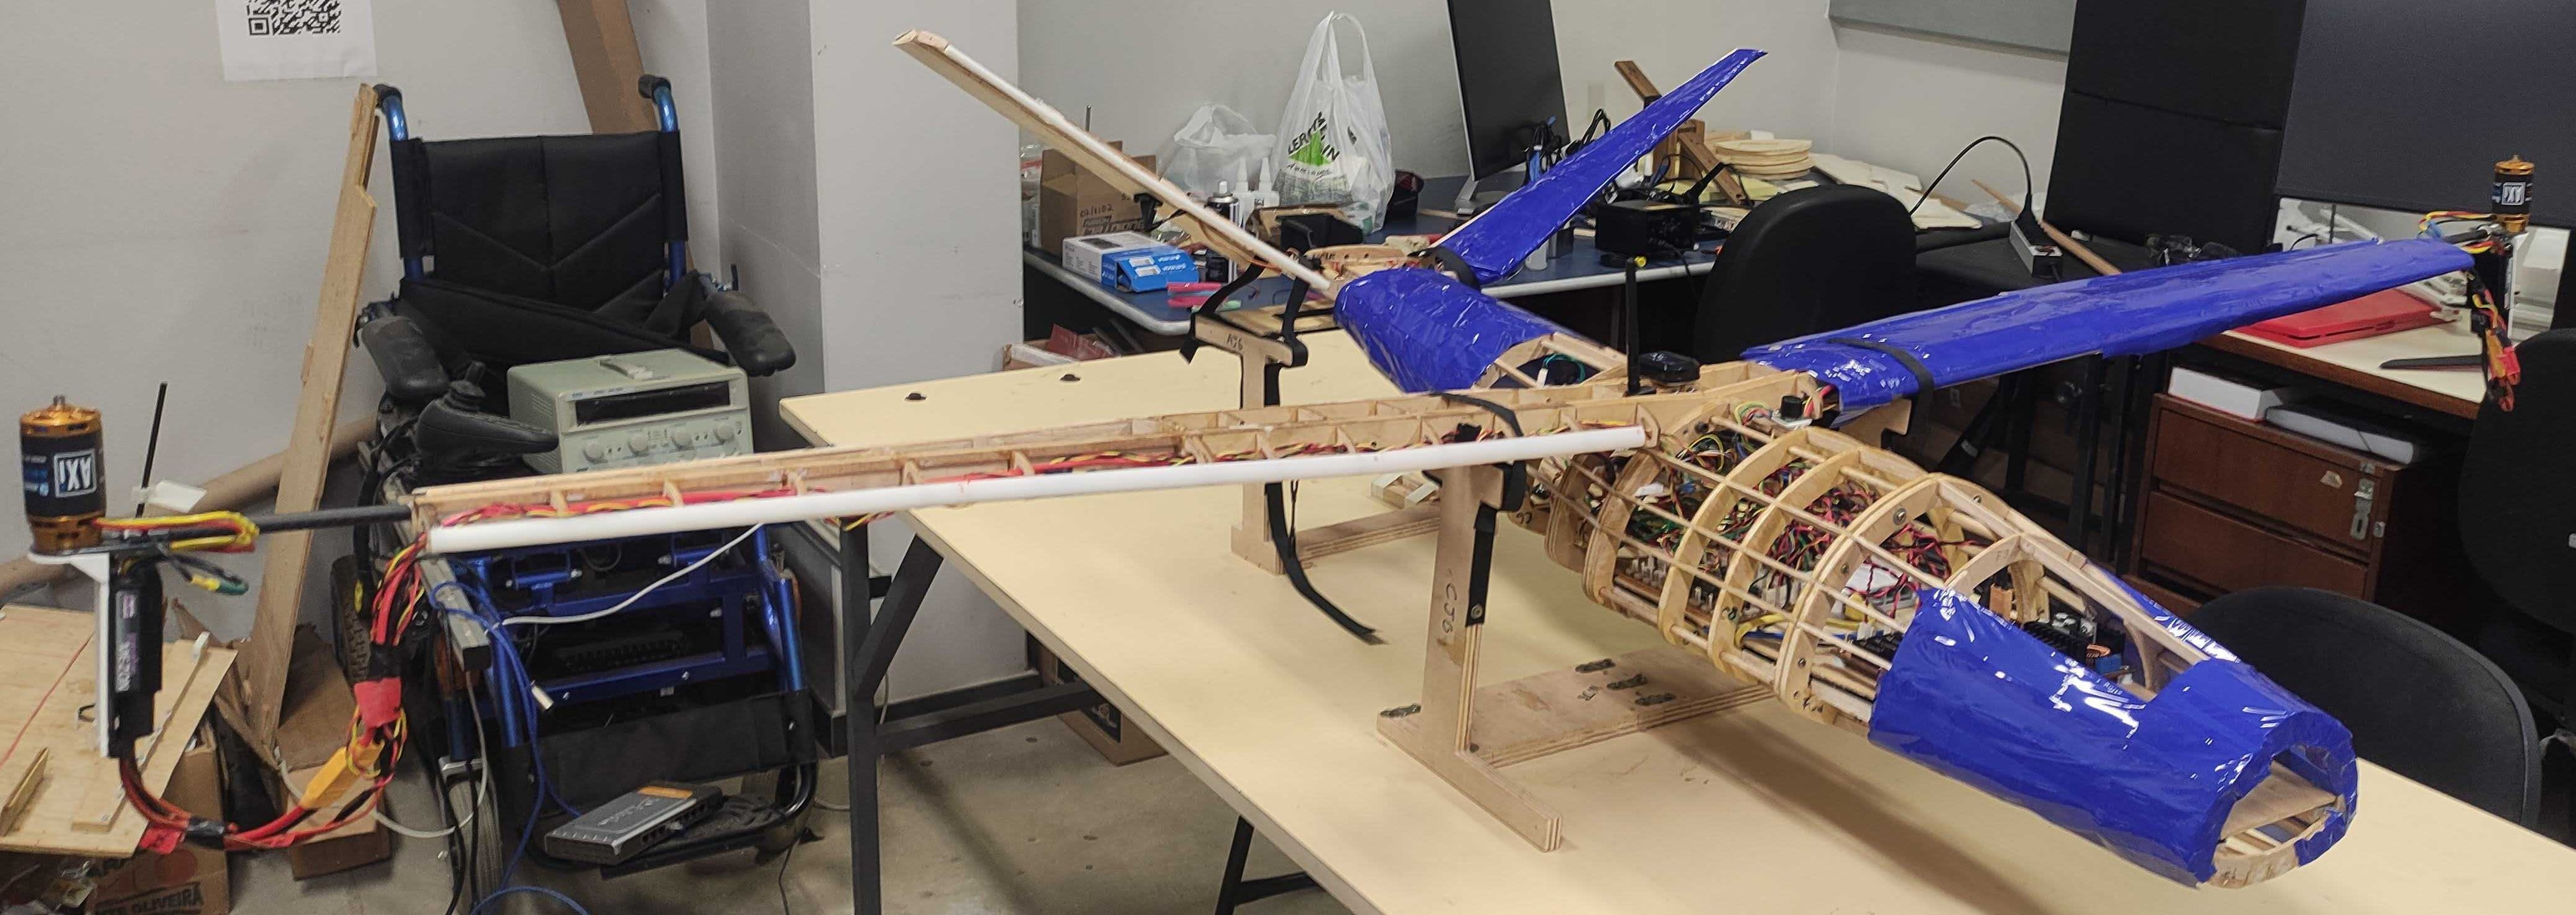
\includegraphics[width=\linewidth]{Figuras/foto-vant4.jpg}
        \caption{Eletrônica embarcada montada no \textit{ProVANT-Emergentia}.}
        \label{fig:vant4}
    \end{figure}

    Com respeito ao desenvolvimento de software, a implementação foi iniciada com o subsistema Nucleo, desenvolvendo os \textit{drivers} dos sensores e atuadores conectados a este computador de bordo. A etapa seguinte consistiu na arquitetura de programa dos computadores e na comunicação Ethernet com o protocolo \textit{Token Ring}, de forma a integrar o sistema. Finalmente, foi feito o desenvolvimento de \textit{drivers} específicos dos subsistemas Raspberry e Jetson.

  \end{block}
\vspace{-1em}
  \begin{block}{Considerações finais}
   Neste trabalho, foi possível projetar um sistema de eletrônica embarcada para um VANT tilt-rotor e implementá-lo de forma a obter um sistema funcional de sensoriamento, atuação e troca de dados. O sistema embarcado do ProVANT-\textit{Emergentia} ainda se encontra em processo de desenvolvimento, de forma que as principais tarefas restantes são: i) Implementação de alguns \textit{drivers} pendentes: servo motores, sensores de alta precisão; ii) Implementação dos algoritmos de controle e estimação; e iii) Validação do sistema completamente integrado.
  \end{block}
  \vspace{-1em}
  \begin{block}{Agradecimentos}
    {\small
    Este trabalho foi financiado pelo INCT-InSAC - Código de financiamento CNPq 465755/2014-3 e pelas agências de fomento FAPESP - Código de Financiamento 2014/50851-0, CNPq - Códigos de Financiamento 304032/2019-0, 317058/2023-1 e 422143/2023-5, FAPEMIG - Código de Financiamento APQ-03090-17 e FUNDEP.}      
  \end{block}
  \vspace{-1em}
  \begin{block}{Referências}
    \nocite{*}
    \vspace{-0.3em}
    {\small
    \bibliographystyle{ieeetr}\bibliography{poster}
    }
  \end{block}

\end{column}
\separatorcolumn



\end{columns}
\end{frame}

\end{document}
